% =====================================================================
%  Laborbericht 1 – Biosignalverarbeitung
%  Aufbau der Hardware & Datenakquise
%  Basierend auf der MCI-LaTeX-Vorlage (Drauschke/Teschl/Mehrle),
%  eigenständig kompilierbar (alle Definitionen in dieser Datei).
%
%  ROT markierte Stellen (\todo{...}) müssen noch ergänzt werden!
%  Max. 10 Seiten – vor der Abgabe Seitenzahl prüfen.
% =====================================================================

\documentclass[a4paper,oneside,10pt]{article}

\usepackage{ifthen}
\newboolean{english}
%\setboolean{english}{true}

% ---------------- Pakete & Layout (aus definitions.tex der Vorlage) ----
% Deutsche Silbentrennung: babel/ngerman bevorzugt, sonst Paket "german" der Vorlage
\IfFileExists{ngerman.ldf}{\usepackage[ngerman]{babel}}{%
  \IfFileExists{german.sty}{\usepackage{german}}{}}
\usepackage[T1]{fontenc}
\usepackage{lmodern}
\setlength{\emergencystretch}{2em}
\usepackage{graphicx}
\graphicspath{{abbildungen/}{../Abgabe_Lab1/figures/}}
\usepackage[tmargin=1in,bmargin=1in,lmargin=1.25in,rmargin=1.25in]{geometry}
\usepackage{titlesec}
\usepackage{xcolor}
\usepackage[overload]{textcase}
\definecolor{MSBlue}{rgb}{.204,.353,.541}
\definecolor{MSLightBlue}{rgb}{.31,.506,.741}
\titleformat{\section}[hang]{\rmfamily\bfseries\huge\color{MSBlue}}{\thesection}{1em}{\MakeLowercase}[]
\titleformat{\subsection}{\large\bfseries\sffamily\uppercase}{\thesubsection}{1em}{}
\titleformat{\subsubsection}{\sffamily\bfseries}{\thesubsubsection}{1em}{}
\def\litname{literatur}
\AtBeginDocument{%
  \renewcommand\contentsname{inhaltsverzeichnis.}%
  \renewcommand\listfigurename{abbildungsverzeichnis.}%
  \renewcommand\listtablename{tabellenverzeichnis.}%
  \renewcommand\refname{\litname.}%
  \renewcommand\figurename{Abbildung}%
  \renewcommand\tablename{Tabelle}}
\usepackage{fancyhdr}
\usepackage[small]{caption}
\usepackage{float}
\usepackage{amsmath,amssymb}
\usepackage{booktabs}
\usepackage{listings}
\setlength{\parindent}{0em}
\setlength{\parskip}{1.2ex plus0.5ex minus0.5ex}
\setlength{\captionmargin}{3em}

\lstset{basicstyle=\ttfamily\footnotesize,frame=single,columns=fullflexible,
        keywordstyle=\bfseries,language=C++,breaklines=true}

% ---------------- Platzhalter-Befehle --------------------------------
% \todo{Text}        -> roter Hinweis im Fließtext
% \platzhalter{Text} -> roter Rahmen anstelle einer noch fehlenden Abbildung
\newcommand{\todo}[1]{\textcolor{red}{\textbf{[TODO:} #1\textbf{]}}}
\newcommand{\platzhalter}[1]{%
  \fcolorbox{red}{white}{\parbox[c][4.2cm][c]{0.85\textwidth}{\centering
  \textcolor{red}{\textbf{PLATZHALTER -- Abbildung noch einfügen}}\\[1ex]
  \textcolor{red}{\small #1}}}}

% ---------------- Angaben Deckblatt ----------------------------------
\def\labtitle{Biosignalverarbeitung Laborbericht}
\def\labcode{BA-MGST-B-3-BB-BS-ILV}
\def\labname{Aufbau der Hardware \& Datenakquise}
\def\labnum{1}
\def\study{Medizin- Sport- und Gesundheitstechnik}
\def\term{3.}
\def\lecturer{Aitor Morillo}
\def\group{MGST-25}
\def\gruppennr{\textcolor{red}{X}} % TODO: Gruppennummer eintragen
\def\student{Matthias Zoller, Laurenz Keller, Matteo Harrasser}

\begin{document}

% =====================================================================
%  Deckblatt (aus deckblatt.tex)
% =====================================================================
\pagestyle{plain}
\thispagestyle{empty}
{\sffamily\bfseries
\vspace*{1cm}

\textcolor{MSBlue}{\rmfamily\bfseries\huge laborbericht.}

\vspace*{0.5cm}
\textbf{\labtitle{ }(\labcode)}

\labname

Labor \labnum{} -- Gruppe \gruppennr

\vspace*{10cm}
\textcolor{gray}{\study}

\textcolor{gray}{\term{ }Semester}

\textcolor{gray}{Lehrveranstaltungsleiter: \lecturer}

\textcolor{gray}{Jahrgang: \group}

\textcolor{gray}{Verfasser: \student}

\textcolor{gray}{\number\day.\,\number\month.\,\number\year}
\newpage}

\tableofcontents
\listoffigures
\listoftables
\newpage

\pagestyle{fancy}
\fancyhf{}
\fancyhead[L]{\small Laborbericht \labnum{} -- \labname}
\fancyhead[R]{\small Gruppe \gruppennr}
\fancyfoot[C]{\thepage}

% =====================================================================
\section{Einleitung}
% =====================================================================
Ziel des ersten Labors ist der Aufbau eines Messsystems zur Erfassung von
Beschleunigungsdaten sowie deren Verarbeitung in Python. Dazu wird der
3-Achsen-Beschleunigungssensor BMA400 über I\textsuperscript{2}C an einen
Arduino Uno angebunden, die Daten über die serielle Schnittstelle an einen PC
übertragen und anschließend in Python eingelesen, gefiltert und dargestellt.
Untersucht werden insbesondere der Einfluss der Datenrate (ODR) des Sensors auf
die Qualität der Messdaten, die tatsächlich erreichte Abtastfrequenz sowie der
Unterschied zwischen stationärem (USB) und mobilem (DataLogger, Batterie)
Messsystem.

Der Python-Code \texttt{MainCode1.ipynb} bearbeitet die Aufgaben 4\,(a), 5,
6\,(a), 7, 8, 9 und 10 und erzeugt alle Abbildungen dieses Berichts.

% =====================================================================
\section{Aufbau des Messsystems (Aufgabe 1)}
% =====================================================================
Abbildung~\ref{fig:messsystem} zeigt das stationäre Messsystem mit allen
Komponenten, Bussen und Signalpfaden.

\begin{figure}[H]
    \centering
    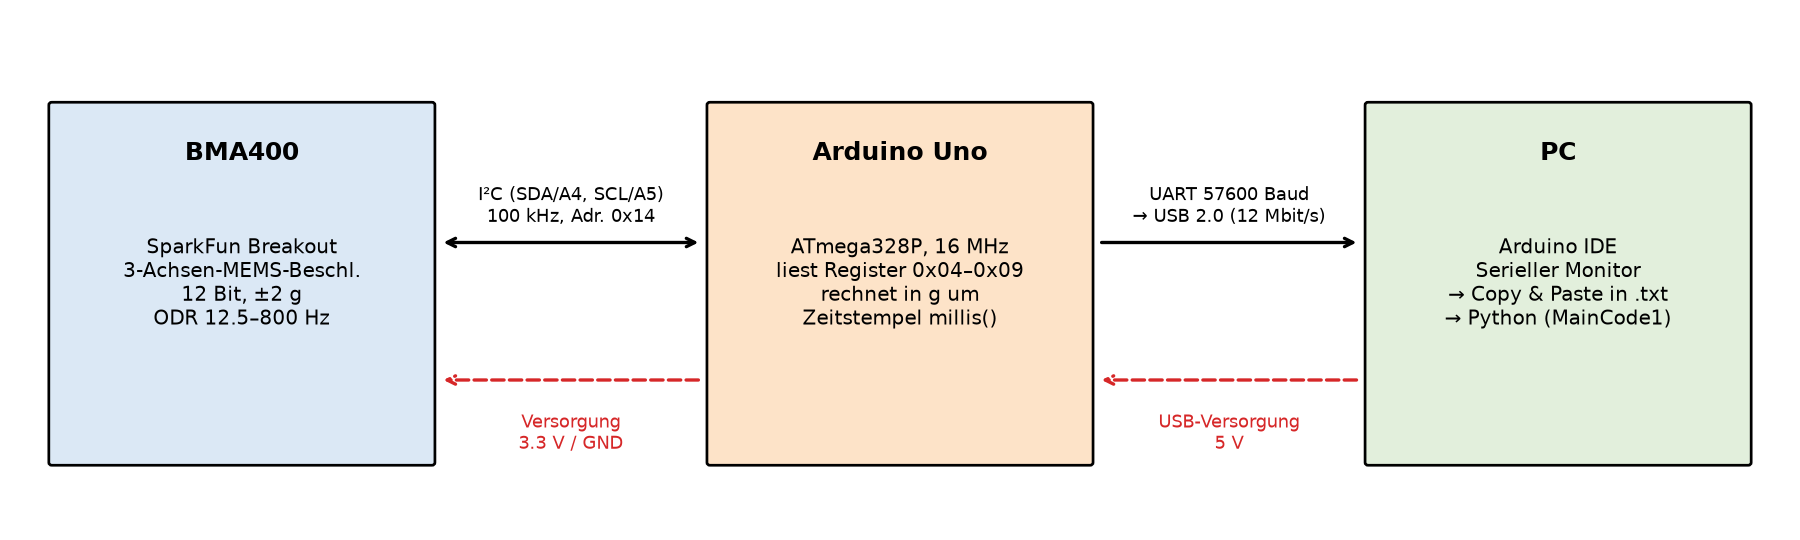
\includegraphics[width=\textwidth]{A1_Messsystem.png}
    \caption{Aufbau des stationären Messsystems. Schwarz: Datenpfade, rot gestrichelt: Spannungsversorgung.}
    \label{fig:messsystem}
\end{figure}

\subsection*{Komponenten}
\begin{description}
    \item[BMA400 (SparkFun Breakout):] Digitaler 3-Achsen-MEMS-Beschleunigungssensor mit
    12~Bit Auflösung. Messbereich ($\pm 2$ bis $\pm 16\,g$) und Datenrate (ODR, 12{,}5--800\,Hz)
    sind einstellbar; die Messwerte stehen in den Registern 0x04--0x09.
    \item[Arduino Uno (ATmega328P, 16\,MHz):] Konfiguriert den Sensor, liest die sechs
    Datenregister aus, rechnet die Rohwerte in $g$ um und hängt den Zeitstempel
    \texttt{millis()} an. Er versorgt den Sensor mit 3{,}3\,V.
    \item[PC (Arduino IDE):] Der serielle Monitor zeigt die Messwerte zeilenweise
    (\texttt{X Y Z Time}) an; sie werden per Copy \& Paste in eine \texttt{.txt}-Datei
    übernommen.
    \item[Python (\texttt{MainCode1.ipynb}):] Liest die Textdatei mit \texttt{pandas} ein,
    filtert mit \texttt{SciPy} und stellt die Daten mit \texttt{matplotlib} dar.
\end{description}

\subsection*{Busse und Signalpfade}
\begin{description}
    \item[I\textsuperscript{2}C (100\,kHz):] Zweidraht-Bus (SDA = A4, SCL = A5). Der Arduino ist
    Master, der Sensor Slave mit der Adresse 0x14.
    \item[UART / USB 2.0:] Der Arduino sendet seriell mit 57\,600\,Baud; ein USB-Seriell-Wandler
    auf dem Board setzt dies auf USB 2.0 Full Speed (12\,Mbit/s) um.
    \item[Datenpfad PC $\rightarrow$ Python:] Übergabe der Messdaten als Textdatei.
    \item[Spannungsversorgung:] 5\,V über USB für den Arduino, 3{,}3\,V und GND vom Arduino
    zum Sensor.
\end{description}

% =====================================================================
\section{Vorausgehende Arbeiten und Berechnungen}
% =====================================================================

\subsection{Umrechnung eines ADC-Wertes in eine Temperatur (Aufgabe 2)}

Gegeben sind ein Temperatursensor mit $U = 0 \ldots 3{,}3$\,V für
$\vartheta = 0 \ldots 40\,^\circ$C (linear) und ein ADC mit $n = 10$\,Bit
($0 \ldots 1023$) und Referenzspannung $U_\mathrm{ref} = 5$\,V. Der ADC liefert
$D = 520$.

\textbf{Schritt 1 -- ADC-Wert in Spannung:}
\begin{equation}
  U = \frac{D}{2^{n}-1}\cdot U_\mathrm{ref} = \frac{520}{1023}\cdot 5\,\mathrm{V} \approx 2{,}542\,\mathrm{V}
\end{equation}

\textbf{Schritt 2 -- Spannung in Temperatur:}
\begin{equation}
  \vartheta = \frac{U}{3{,}3\,\mathrm{V}}\cdot 40\,^\circ\mathrm{C}
            = \frac{2{,}542\,\mathrm{V}}{3{,}3\,\mathrm{V}}\cdot 40\,^\circ\mathrm{C}
            \approx \mathbf{30{,}8\,^\circ C}
\end{equation}

Der Sensor misst also ca.\ 30{,}8\,°C, was für eine Messung auf der Haut plausibel
ist (die Hauttemperatur liegt unter der Körperkerntemperatur von ca.\ 37\,°C).
Da der Sensor höchstens 3{,}3\,V liefert, werden nur ADC-Werte bis
$\frac{3{,}3}{5}\cdot 1023 \approx 675$ genutzt; die Auflösung beträgt damit
$40\,^\circ\mathrm{C}/675 \approx 0{,}06\,^\circ$C pro Stufe statt der möglichen
$0{,}04\,^\circ$C.

\subsection{Achsenzuordnung und Umrechnung in physikalische Größen (Aufgabe 3)}

\textbf{Achsenzuordnung:} \texttt{Lab1Code1} gibt pro Zeile \texttt{X Y Z Time}
aus; die Spalten entsprechen der Reihenfolge der Datenregister (0x04/0x05 = $x$,
0x06/0x07 = $y$, 0x08/0x09 = $z$) und damit den auf der Platine aufgedruckten Achsen.

\textbf{Test:} Der Sensor wird so hingelegt, dass eine Achse senkrecht nach oben
zeigt. Diese Achse zeigt dann ca.\ $+1\,g$, die anderen ca.\ $0\,g$. Flach auf dem
Tisch ($z$ nach oben) wurde z.\,B.\ \texttt{7 -91 1002} gemessen, also $z \approx 1\,g$.
Die systematische Prüfung aller sechs Lagen erfolgt in Aufgabe~6.

\textbf{Einheit:} Ausgegeben werden Rohwerte in LSB (Digits): pro Achse zwei
Register (LSB, MSB), die zusammen einen 12-Bit-Wert im Zweierkomplement
($-2048 \ldots +2047$) ergeben:
\texttt{raw = ((msb \& 0x0F) << 8) | lsb}, danach bei \texttt{raw > 2047}
$\rightarrow$ \texttt{raw -= 4096}.

\textbf{Umrechnung:} Die Empfindlichkeit ergibt sich laut Datenblatt \cite{bma400}
\todo{Seite/Tabelle der Sensitivity eintragen} zu
$S = 2048/\text{Messbereich}$, also $S = 1024$\,LSB/$g$ bei $\pm 2\,g$:
\begin{equation}
  a\,[g] = \frac{\text{raw}}{1024}, \qquad
  a\,[\mathrm{m/s^2}] = \frac{\text{raw}}{1024}\cdot 9{,}81\,\mathrm{m/s^2}
\end{equation}
Beispiel: $1002/1024 = 0{,}98\,g = 9{,}60$\,m/s$^2$.

% =====================================================================
\section{Durchführung und Ergebnisse}
% =====================================================================

\subsection{Auf- und Abbewegung mit dem Originalcode (Aufgabe 4)}

Der Sensor wurde in der geschlossenen Hand gehalten und ca.\ einmal pro Sekunde
schnell auf und ab bewegt (ohne Rotation). Die Daten wurden mit \texttt{Lab1Code1}
(ODR 12{,}5\,Hz, $\pm 2\,g$) aufgezeichnet und in eine Textdatei kopiert.

\textbf{(a)} Abbildung~\ref{fig:a4} zeigt 4\,s der Messung, umgerechnet in $g$.

\begin{figure}[H]
  \centering
  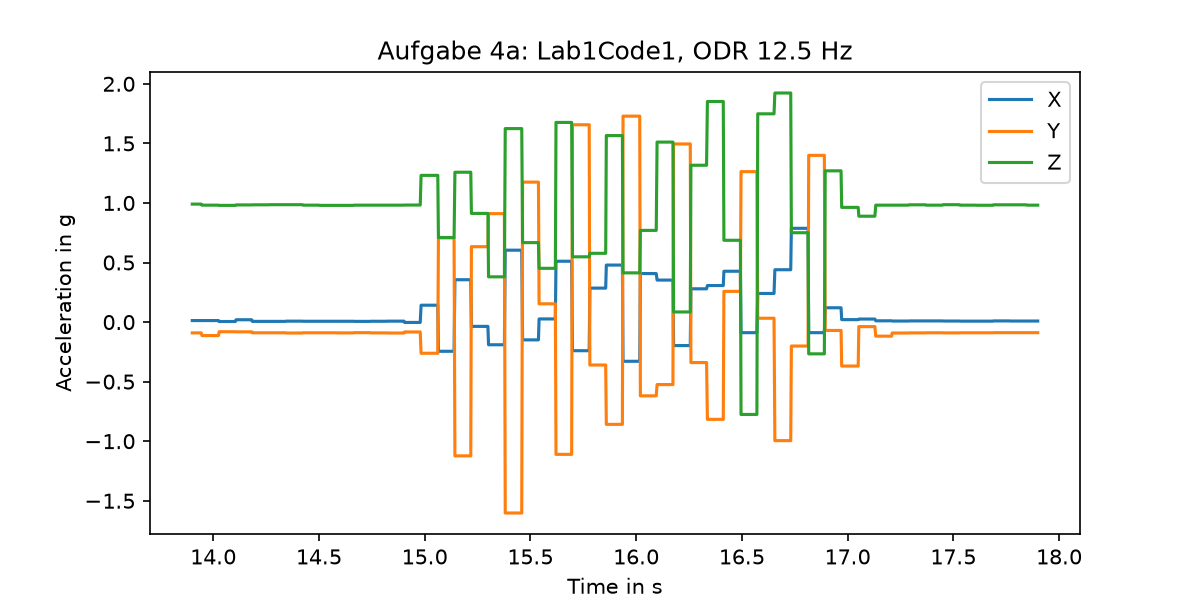
\includegraphics[width=0.85\textwidth]{A4a_12_5Hz.png}
  \caption{Auf- und Abbewegung mit \texttt{Lab1Code1} (ODR 12{,}5\,Hz), Ausschnitt 4\,s.}
  \label{fig:a4}
\end{figure}

\textbf{(b) Plateaus der Peaks:} Jeder Wert bleibt ca.\ 80\,ms konstant, wodurch
die treppenförmigen Plateaus entstehen. Der Sensor liefert neue Werte nur mit der
ODR von 12{,}5\,Hz (alle 80\,ms), die \texttt{loop()} gibt ohne \texttt{delay}
jedoch ca.\ alle 3\,ms ($\approx 313$\,Hz, vgl.\ Tab.~\ref{tab:fs}) eine Zeile aus.
Bis ein neuer Wert im Datenregister steht, wird also immer wieder derselbe Wert
gelesen (ca.\ 25 identische Zeilen pro Messwert). \textbf{Lösung:} Die ODR im
Register \texttt{ACC\_CONFIG1} erhöhen (Aufgabe~5) und die Ausgaberate mit einem
passenden \texttt{delay} an die ODR anpassen. Zusätzlich liegen die Peaks in $z$
(inkl.\ Erdbeschleunigung) mit ca.\ $1{,}9\,g$ nahe an der Messbereichsgrenze von
$\pm 2\,g$; für stärkere Bewegungen sollte daher auch der Messbereich vergrößert
werden, um Sättigung zu vermeiden.

\textbf{(c) Abweichung von der tatsächlichen Bewegung:} Bei 12{,}5\,Hz liegt die
Nyquist-Frequenz bei 6{,}25\,Hz. Die schnelle Bewegung enthält höhere
Frequenzanteile, sodass \emph{Aliasing} entsteht: Pro Bewegung gibt es nur wenige
Messpunkte, das Signal springt (v.\,a.\ in $y$) fast bei jedem Sample das Vorzeichen,
statt den Bewegungsverlauf zu zeigen. Außerdem misst der Sensor immer die
Erdbeschleunigung mit; dreht sich die Hand leicht, verteilt sich diese auf
mehrere Achsen.

\subsection{Anpassung der Sensorkonfiguration (Aufgabe 5)}

Die Datenrate wird laut Datenblatt BMA400 \cite{bma400} (Rev.~2.3, \textbf{S.~64})
im Register \texttt{ACC\_CONFIG1} (0x1A) über den Parameter \texttt{acc\_odr}
(Bits 3:0) eingestellt. Die möglichen Werte zeigt Tab.~\ref{tab:odr}.

\begin{table}[H]
\centering
\small
\caption{Mögliche Werte des Parameters \texttt{acc\_odr} im Register \texttt{ACC\_CONFIG1} (0x1A) des BMA400.}
\label{tab:odr}
\begin{tabular}{lccccccccc}
\toprule
\texttt{acc\_odr} & 0x00--0x04 & 0x05 & 0x06 & 0x07 & \textbf{0x08} & 0x09 & 0x0A & 0x0B & 0x0C--0x0F \\
\midrule
ODR / Hz & reserviert & 12{,}5 & 25 & 50 & \textbf{100} & 200 & 400 & 800 & reserviert \\
\bottomrule
\end{tabular}
\end{table}

Im Code (\texttt{Lab1Code1\_modifiziert.ino}) wurden folgende Zeilen geändert:
\begin{lstlisting}
accel.setODR(BMA400_ODR_100HZ);   // ACC_CONFIG1 (0x1A), acc_odr = 0x08
...
delay(10);                        // Ausgaberate an ODR anpassen: 1/100 Hz = 10 ms
\end{lstlisting}

\textbf{Begründung:} Handbewegungen liegen deutlich unter 50\,Hz (Nyquist-Frequenz
bei 100\,Hz) und werden damit ohne Aliasing erfasst. Höhere Raten sind nicht
sinnvoll: Eine Ausgabezeile (\texttt{-0.1234\textbackslash t} $\times 3$ + Zeitstempel
+ Zeilenumbruch) umfasst ca.\ 30 Zeichen $\approx 300$\,Bit, bei 57\,600\,Baud sind
also nur ca.\ 190 Zeilen/s übertragbar -- 200\,Hz und mehr würden die serielle
Schnittstelle überlasten.

\begin{figure}[H]
  \centering
  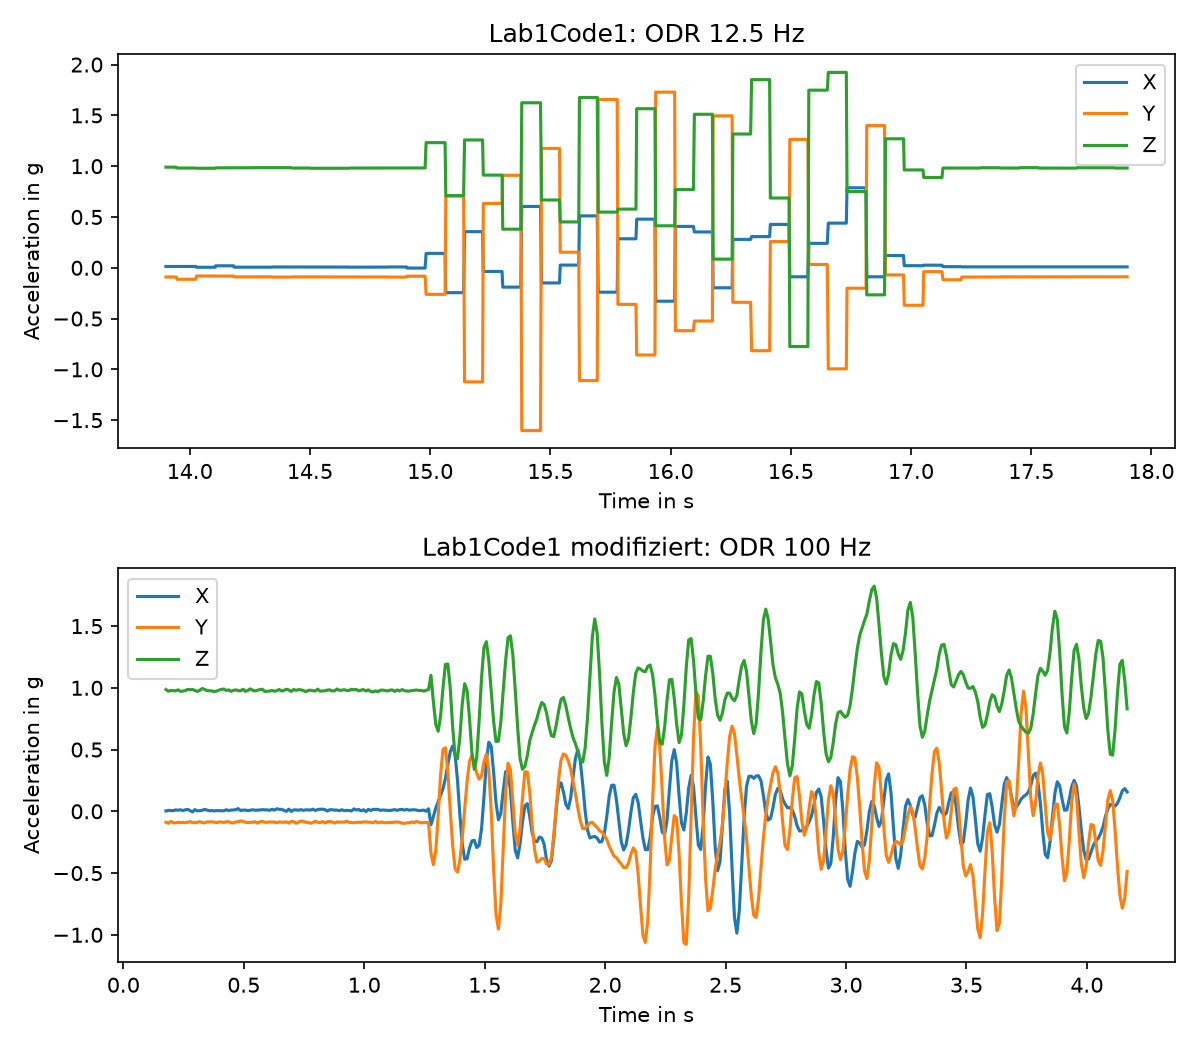
\includegraphics[width=0.72\textwidth]{A5_Vergleich_12_5Hz_100Hz.png}
  \caption{Vergleich je 4\,s: oben ODR 12{,}5\,Hz (\texttt{Lab1Code1}), unten ODR 100\,Hz (modifizierter Code).}
  \label{fig:a5}
\end{figure}

\textbf{Vergleich (Abb.~\ref{fig:a5}):} Gleich sind der Ruhepegel ($z \approx 1\,g$,
$x$ und $y \approx 0$) und die Größenordnung der Ausschläge (bis ca.\ $1{,}8\,g$).
Bei 100\,Hz gibt es jedoch keine Treppenstufen mehr: Die Kurve ist glatt und die
einzelnen Auf-ab-Bewegungen sind als Schwingung zu erkennen, während das Signal bei
12{,}5\,Hz durch das Aliasing zerhackt ist. Ursache ist ausschließlich die höhere
Abtastrate; Sensor und Messbereich sind gleich geblieben.

\subsection{Zeitstempel und statische Messung in sechs Orientierungen (Aufgabe 6)}

Jede Zeile erhält direkt auf dem Arduino den Zeitstempel \texttt{millis()}
(4.~Spalte), unabhängig von den Zeitstempeln des seriellen Monitors. Daraus wird in
Abschnitt~\ref{sec:fs} die mittlere Abtastfrequenz berechnet. Der Sensor wurde
nacheinander in alle sechs Lagen gebracht und jeweils ca.\ 10\,s ruhig gehalten.

\textbf{(a)} Abbildung~\ref{fig:a6} zeigt die gesamte Messung.

\begin{figure}[H]
  \centering
  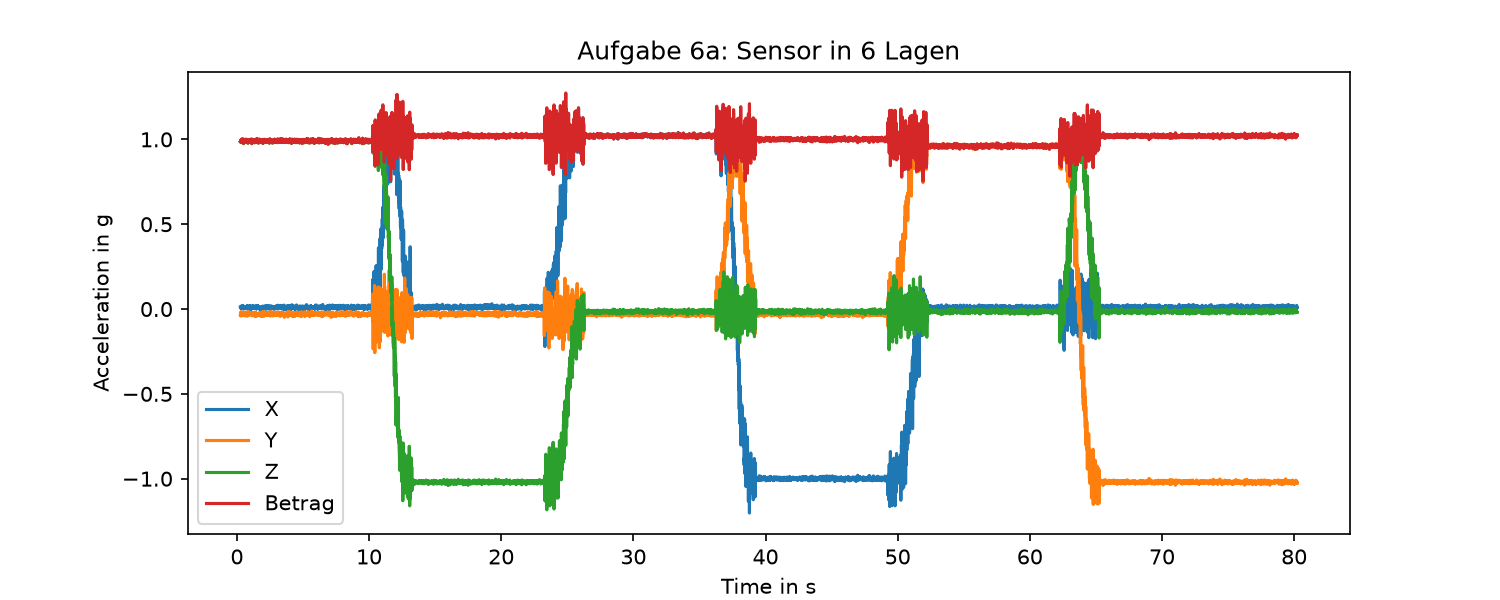
\includegraphics[width=0.9\textwidth]{A6a_6_Lagen.png}
  \caption{Sensor in sechs Lagen à ca.\ 10\,s; rot: Betrag $|a| = \sqrt{x^2+y^2+z^2}$.}
  \label{fig:a6}
\end{figure}

\textbf{(b) Plausibilität:} Tabelle~\ref{tab:lagen} zeigt die Mittelwerte in den
Ruhephasen.

\begin{table}[H]
\centering
\small
\caption{Mittelwerte der Beschleunigung in den sechs Lagen (Werte in $g$).}
\label{tab:lagen}
\begin{tabular}{lcccc}
\toprule
Lage & $x$ & $y$ & $z$ & $|a|$ \\
\midrule
$z$ oben  & 0{,}01 & $-0{,}03$ & \textbf{0{,}99} & 0{,}99 \\
$z$ unten & 0{,}01 & $-0{,}03$ & \textbf{$-$1{,}02} & 1{,}02 \\
$x$ oben  & \textbf{1{,}02} & $-0{,}03$ & $-0{,}02$ & 1{,}02 \\
$x$ unten & \textbf{$-$1{,}00} & $-0{,}03$ & $-0{,}02$ & 1{,}00 \\
$y$ oben  & 0{,}01 & \textbf{0{,}96} & $-0{,}02$ & 0{,}96 \\
$y$ unten & 0{,}01 & \textbf{$-$1{,}02} & $-0{,}02$ & 1{,}02 \\
\bottomrule
\end{tabular}
\end{table}

Die Daten ergeben Sinn: Die senkrecht stehende Achse zeigt immer ca.\ $\pm 1\,g$,
die anderen ca.\ $0\,g$, und der Betrag liegt stets bei ca.\ $1\,g$. Zeigt eine Achse
nach oben, ist der Wert positiv, weil der Sensor die Gegenkraft der Unterlage
misst. Die kleinen Abweichungen (bis 0{,}04\,$g$) entstehen durch Offset-Fehler
des Sensors und dadurch, dass er von Hand nicht exakt gerade gehalten wurde.

\subsection{Filterung der Daten (Aufgabe 7)}

Die Daten aus Aufgabe~6 wurden mit einem Butterworth-Tiefpass 4.~Ordnung mit der
Grenzfrequenz $f_g = 5$\,Hz gefiltert. Dabei wurde \texttt{filtfilt()} aus
\texttt{scipy.signal} \cite{scipy} verwendet, das den Filter vorwärts und rückwärts
anwendet und so keine Phasenverschiebung erzeugt (Nullphasenfilter).

\begin{figure}[H]
  \centering
  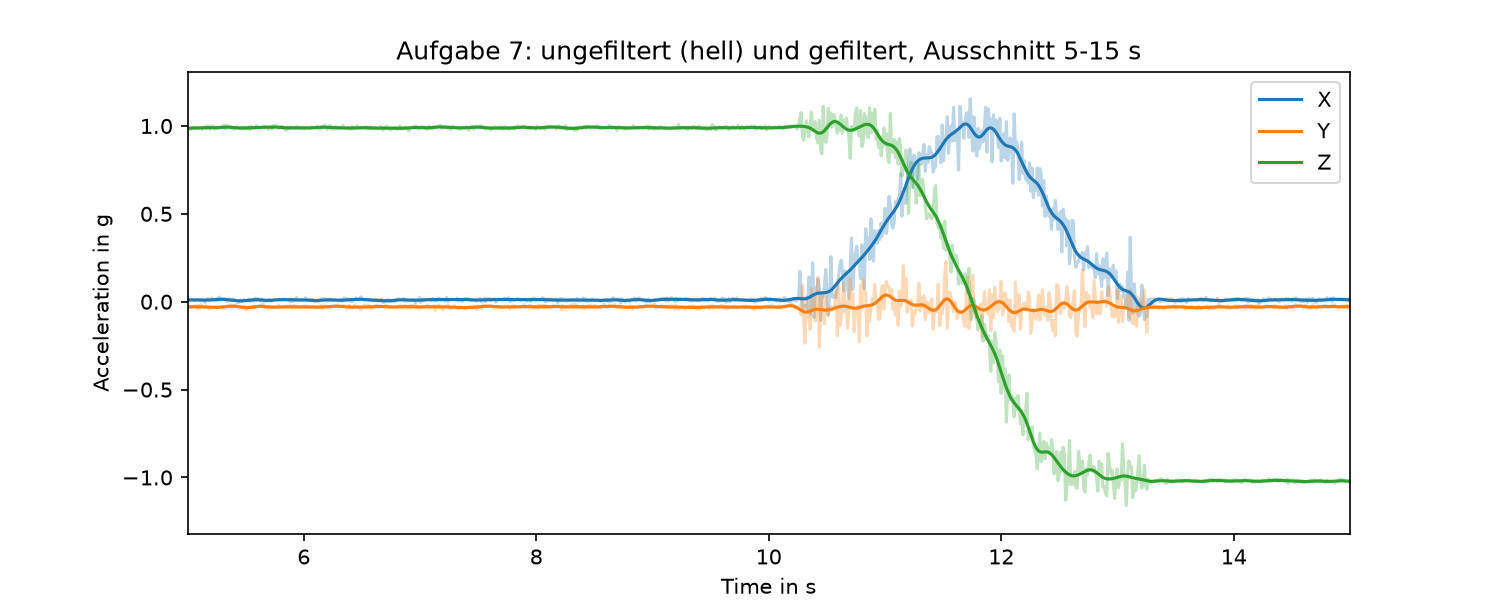
\includegraphics[width=0.9\textwidth]{A7_Filter.png}
  \caption{Ungefilterte (hell) und tiefpassgefilterte Daten ($f_g = 5$\,Hz), Ausschnitt 5--15\,s.}
  \label{fig:a7}
\end{figure}

\textbf{Effekt und Begründung:} Der Filter entfernt das Sensorrauschen und das
Zittern der Hand (in Ruhe sinkt die Standardabweichung von $z$ von 6{,}0 auf
1{,}6\,m$g$), während die Lagewechsel erhalten bleiben und durch \texttt{filtfilt}
nicht verschoben werden (Abb.~\ref{fig:a7}). Ein Tiefpass wurde gewählt, weil sich
die Lage nur langsam ändert, das Rauschen aber hochfrequent ist.

\subsection{Bestimmung der Abtastfrequenz (Aufgabe 8)}
\label{sec:fs}

Aus den \texttt{millis()}-Zeitstempeln wurden die Abtastintervalle
$\Delta t_i = t_{i+1}-t_i$ und daraus
\begin{equation}
  \bar f_s = \frac{1}{\overline{\Delta t}}, \qquad
  \sigma_{f_s} \approx \frac{\sigma_{\Delta t}}{\overline{\Delta t}^{\,2}}
\end{equation}
bestimmt (Fehlerfortpflanzung). Abbildung~\ref{fig:a8} zeigt die Verteilung der
Intervalle, Tab.~\ref{tab:fs} die Ergebnisse.

\begin{figure}[H]
  \centering
  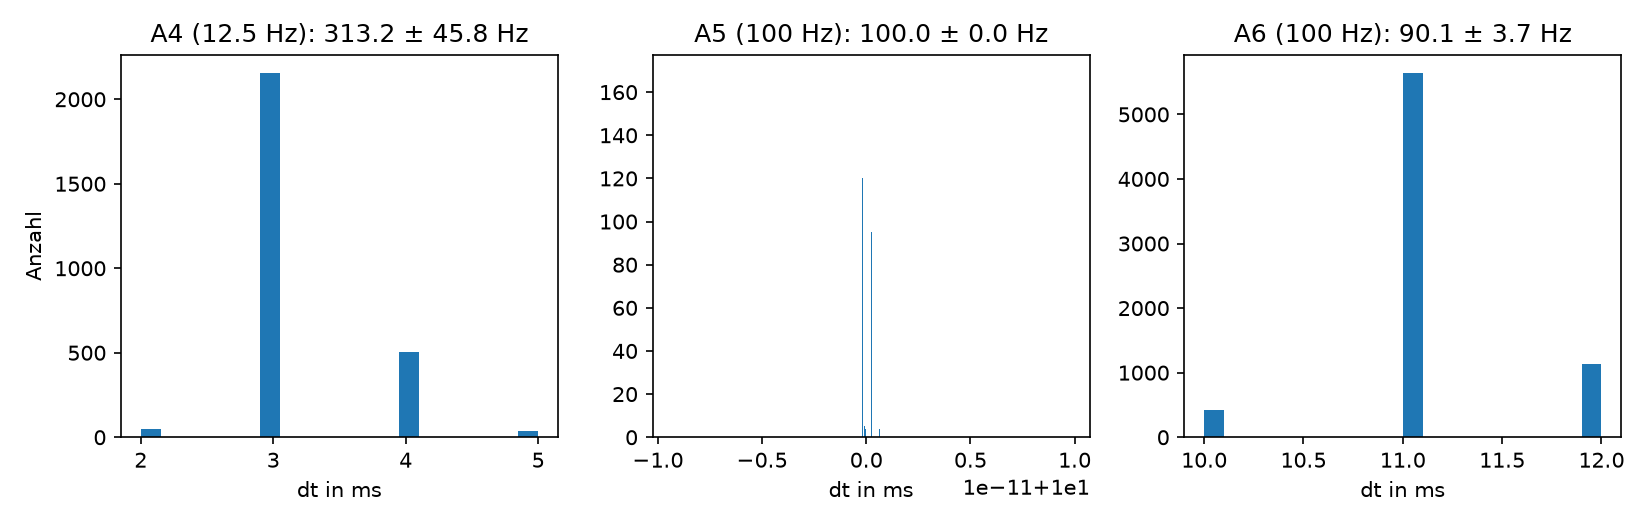
\includegraphics[width=\textwidth]{A8_Abtastfrequenz.png}
  \caption{Histogramme der Abtastintervalle $\Delta t$ der drei Messungen.}
  \label{fig:a8}
\end{figure}

\begin{table}[H]
\centering
\small
\caption{Abtastintervalle und Abtastfrequenzen der Messungen.}
\label{tab:fs}
\begin{tabular}{lccc}
\toprule
Messung & $\overline{\Delta t}$ / ms & $\sigma_{\Delta t}$ / ms & $\bar f_s$ / Hz \\
\midrule
A4: \texttt{Lab1Code1} (ODR 12{,}5\,Hz)        & 3{,}19  & 0{,}47 & $313 \pm 46$ \\
A5: modifiziert (ODR 100\,Hz)                   & 10{,}00 & 0{,}00 & $100{,}0 \pm 0{,}0$ \\
A6: 6 Lagen (ODR 100\,Hz)                       & 11{,}10 & 0{,}46 & $90{,}1 \pm 3{,}7$ \\
A9: mobiles System (\texttt{Lab1Code2})         & \todo{?} & \todo{?} & \todo{?} \\
\bottomrule
\end{tabular}
\end{table}

Bei \texttt{Lab1Code1} gibt die Schleife ohne \texttt{delay} mit ca.\ 313\,Hz aus,
neue Sensorwerte kommen aber nur mit 12{,}5\,Hz. Mit dem geänderten Code passen
Ausgabe und ODR zusammen und die Abtastfrequenz liegt bei ca.\ 100\,Hz. Sie liegt in
Messung A6 etwas darunter (90\,Hz), weil zu \texttt{delay(10)} noch die Zeit für das
Auslesen über I\textsuperscript{2}C und \texttt{Serial.print} hinzukommt
($\Delta t \approx 11$\,ms). Da \texttt{millis()} nur auf 1\,ms genau auflöst, wäre
\texttt{micros()} für eine genauere Bestimmung besser geeignet.
\todo{Messung A5 prüfen: Exakt 10{,}00\,ms bei jedem Sample ($\sigma = 0$) passt nicht zu A6
mit demselben Code (11{,}1\,ms). Wurde A5 mit anderem Code/Timing aufgenommen? Ggf. erklären oder neu messen.}

\subsection{Mobiles Messsystem (Aufgabe 9)}

\todo{Messung mit DataLogger + Batterie und \texttt{Lab1Code2} (ca.\ 10\,s) durchführen,
Ergebnis in Tab.~\ref{tab:fs} eintragen und Text an die Messwerte anpassen.}

Für diese Messung wurde das mobile Messsystem mit DataLogger und Batterie verwendet.
Mit \texttt{Lab1Code2} wurden ca.\ 10\,s aufgezeichnet und die Abtastfrequenz wie in
Abschnitt~\ref{sec:fs} bestimmt (Tab.~\ref{tab:fs}).

\textbf{Diskussion} (Entwurf): Die Abtastfrequenz des mobilen Systems unterscheidet
sich vom stationären Wert und streut stärker. Ursache ist, dass die Daten nicht
mehr nur seriell an den PC ausgegeben, sondern auf eine SD-Karte geschrieben werden.
Das Schreiben erfolgt blockweise und dauert unregelmäßig mehrere Millisekunden, in
denen keine neuen Werte gelesen werden. Zudem unterscheiden sich der verwendete Code
(\texttt{Lab1Code2}, z.\,B.\ Datenrate, Ausgabeformat, \texttt{delay}), die
Übertragungsgeschwindigkeit zum Logger und ggf.\ die Taktquelle. Die eingestellte
ODR stellt daher nur eine Obergrenze dar; die tatsächliche Abtastfrequenz wird von
der langsamsten Stelle der Signalkette bestimmt.

% =====================================================================
\section{Zusammenfassung}
% =====================================================================
Das Messsystem aus BMA400, Arduino Uno und PC wurde aufgebaut und in Betrieb genommen.
Mit der Standardkonfiguration (ODR 12{,}5\,Hz) bildeten die Daten die schnelle
Bewegung wegen zu geringer Abtastrate (Aliasing) und mehrfach ausgegebener Werte
nicht korrekt ab. Durch Erhöhen der ODR auf 100\,Hz im Register \texttt{ACC\_CONFIG1}
und Anpassen der Ausgaberate wurde die Bewegung korrekt erfasst. Die statische Messung
bestätigte in allen sechs Lagen eine Beschleunigung von ca.\ $1\,g$ (Abweichung
$\leq 0{,}04\,g$). Ein Butterworth-Tiefpass (5\,Hz, \texttt{filtfilt}) reduzierte das
Rauschen deutlich ohne Phasenverschiebung. Die tatsächliche Abtastfrequenz betrug
ca.\ 90--100\,Hz (stationär) bzw.\ \todo{?}\,Hz (mobil).

% =====================================================================
\begin{thebibliography}{9}
\bibitem{bma400}
Bosch Sensortec, ``BMA400 -- Ultra-low power triaxial accelerometer,'' Datenblatt,
Rev.~2.3. \todo{Dokumentnummer/Link eintragen.}

\bibitem{sparkfun}
SparkFun Electronics, ``SparkFun Triple Axis Accelerometer Breakout -- BMA400 (Qwiic), Hookup Guide,'' online.
\todo{URL und Abrufdatum}

\bibitem{scipy}
P.~Virtanen \emph{et al.}, ``SciPy 1.0: Fundamental algorithms for scientific computing in Python,''
\emph{Nature Methods}, vol.~17, pp.~261--272, 2020.
\end{thebibliography}

% =====================================================================
\appendix
\section{Anhang: Abgegebene Dateien (Aufgabe 10)}
% =====================================================================
Die Abgabe \texttt{Lab1\_Gruppe\_\gruppennr.zip} enthält:
\begin{itemize}
  \item \texttt{Bericht\_1\_Gruppe\_\gruppennr.pdf} -- dieser Bericht,
  \item \texttt{Lab1Code1\_modifiziert.ino} -- modifizierter Arduino-Code (Aufgabe 5),
  \item \texttt{MainCode1.ipynb} -- Python-Auswertung (Aufgaben 4a, 5, 6a, 7, 8, 9); läuft komplett durch und speichert alle Abbildungen in \texttt{figures/},
  \item Datensätze in \texttt{data/}: \texttt{IMU\_A4\_Lab1Code1\_roh.csv}, \texttt{IMU\_A5\_Lab1Code1mod\_100Hz.csv}, \texttt{IMU\_A6\_Lagen.csv}, \todo{Datensatz Aufgabe 9}.
\end{itemize}

\end{document}
